\documentclass[12pt]{article}
\usepackage[noend]{algpseudocode}
\usepackage{algorithm}
\usepackage{amsthm}
\usepackage{amsmath}
\usepackage{amsfonts}
\usepackage{amssymb}
\usepackage[round]{natbib}
\usepackage{multirow}
\usepackage{stfloats}
\usepackage{fancyhdr}
\usepackage{float}
\usepackage{graphicx}
\usepackage{xcolor}
\usepackage{geometry}
\usepackage{url}
\usepackage[
  bookmarks=false,
  pdfpagelabels=false,
  hyperfootnotes=false,
  hyperindex=false,
  pageanchor=false,
  colorlinks,
  citecolor=blue
]{hyperref}
\usepackage{cleveref}
\usepackage[notref, notcite]{showkeys}

\graphicspath{{../figures/}}
\linespread{1.3}
\bibliographystyle{abbrvnat}
\newcommand\NoDo{\renewcommand\algorithmicdo{}}     % remove "do" from algs

\setlength{\parindent}{0em}
\setlength{\parskip}{.5em}


\pagestyle{fancy}
\setlength{\headheight}{52pt}





\usepackage{titlesec}
\titlespacing{\section}{0ex}{0.5em}{1em}
\titlespacing{\subsection}{0ex}{0.7em}{0.5em}
\titlespacing{\subsubsection}{0ex}{0.7em}{0.5em}
\titleformat*{\section}{\large \bfseries}
\titleformat*{\subsection}{\normalsize \bfseries}
\titleformat*{\subsubsection}{\normalsize \itshape}


\newcommand{\vs}{

    \vspace{0.5em}

}

\newcommand{\E}{\mathbb{E}}             % Expectation
\newcommand{\R}{\mathbb{R}}             % Real numbers
\newcommand{\I}{\mathbb{I}}             % Indicator function
\newcommand{\D}{\mathcal{D}}            % Calligraphic D
\newcommand{\M}{\mathcal{M}}            % Calligraphic M
\newcommand{\Q}{\mathcal{Q}}            % Calligraphic Q
\renewcommand{\S}{\mathcal{S}}          % Calligraphic S
\renewcommand{\L}{\mathcal{L}}          % Calligraphic L
\renewcommand{\P}{\mathbb{P}}          % Calligraphic L
\newcommand{\KL}{\text{KL}}             % KL divergence

\newcommand{\argmin}{{\arg\!\min}}      % arg min without space
\newcommand{\argmax}{{\arg\!\max}}      % arg max without space

\newcommand{\red}[1]{{\color{red} #1}}

\DeclareMathOperator{\card}{card}
\DeclareMathOperator{\corr}{corr}
\DeclareMathOperator{\cov}{cov}
\DeclareMathOperator{\diag}{diag}
\DeclareMathOperator{\rank}{rank}
\DeclareMathOperator{\tr}{tr}
\DeclareMathOperator{\Var}{Var}


\title{Group Sparse Variational Bayes}
\author{}
\date{}

\renewcommand{\red}[1]{\textcolor{red}{#1}}

\begin{document}
\maketitle


\section{Problem formulation}

\subsection{Setting}

Consider the model,
\begin{equation} \label{eq:model} 
    y = \langle x, \beta \rangle + \epsilon
\end{equation}
where $y \in \R$ is the response, $x = (x_1, \dots, x_p)^\top \in \R^p$ a feature vector of explanatory variables, $\beta = (\beta_1, \dots, \beta_p)^\top \in \R^p$ the coefficient vector, and $\epsilon$ a noise term. 

Under a \textit{group-sparse} setting, it is assumed that features can be grouped, and that few groups have non-zero coefficient values \citep{Giraud2021}.  Formally, define the groups as $G_k = \{ G_{k,1}, \dots, G_{k, m_k} \}$ for $k=1,\dots,M$ as disjoint sets of indices such that $ \bigcup_{k=1}^M G_k = \{1, \dots, p \}$ and let $G_k^c = \{1,\dots, p \} \setminus G_k$. Further, denote $x_{G_k} = \{x_j : j \in G_k \}$ and $\beta_{G_k} = \{\beta_j : j \in G_k \}$. 

Under the group structure \eqref{eq:model} can be written as:
\begin{equation}
    y = \left( \sum_{k=1}^{M} \langle x_{G_k}, \beta_{G_k} \rangle \right) + \epsilon
\end{equation}

Furthermore we are going to assume the error term $\epsilon \overset{\text{iid.}}{\sim} N(0, \tau^2)$, under which the log-likelihood is given by,
\begin{align}
    \ell(\D; \beta) = &\ -\frac{1}{2} \sum_{i=1}^n \left[ 
	\log(2\pi \tau^2) + \frac{1}{\tau^2} 
	(y_i - \langle x_i, \beta \rangle)^2
    \right] \nonumber \\
    =&\ - \frac{n}{2}\log(2\pi\tau^2) - \frac{1}{2\tau^2} \| y - X \beta \|^2 \label{eq:log-likelihood}
\end{align}
where $\D = \{ (y_i, x_i) \}_{i=1}^n, y_i \in \R, x_i \in \R^p,  y = (y_1, \dots, y_n)^\top \in \R^n$ and $X = (x_1, \dots, x_n)^\top \in \R^{n \times p}$.


\subsection{Prior}

We consider a group spike-and-slab (GSpSL) prior for the model parameters $\beta$, which has a hierarchical representation,
\begin{equation}
\begin{aligned}
\beta_{G_k} | z_k \overset{\text{ind}}{\sim} &\ z_k \Psi(\beta_{G_k}; \lambda) + (1-z_k) \delta_0(\beta_{G_k}) \\
z_k | \theta_k \overset{\text{ind}}{\sim} &\ \text{Bernoulli}(\theta_k) \\
\theta_k \overset{\text{iid}}{\sim} &\ \text{Beta}(a_0, b_0)
\end{aligned}
\end{equation}
for $k=1,\dots,M$, where $\delta_0$ is the multivariate Dirac mass on zero with dimension $m_k = \dim(\beta_k)$, and $\Psi(\beta_{G_k})$ is the multivariate double exponential distribution with density
\begin{equation} \label{eq:density_mvde}
    \psi(\beta_{G_k}; \lambda) = C_k \lambda^{m_k} \exp \left( - \lambda \| \beta_{G_k} \| \right)
\end{equation}
where $ C_k = \left[ 2^{m_k} \pi^{(m_k -1)/2} \Gamma \left( (m_k + 1) /2 \right) \right]^{-1} $ and $ \| \cdot \| $ is the $\ell_2$-norm. For a visual representation, the density \eqref{eq:density_mvde} for the two-dimensional multivariate double exponential is shown in \Cref{fig:double_exp}.
\begin{figure}[htp]
    \centering
    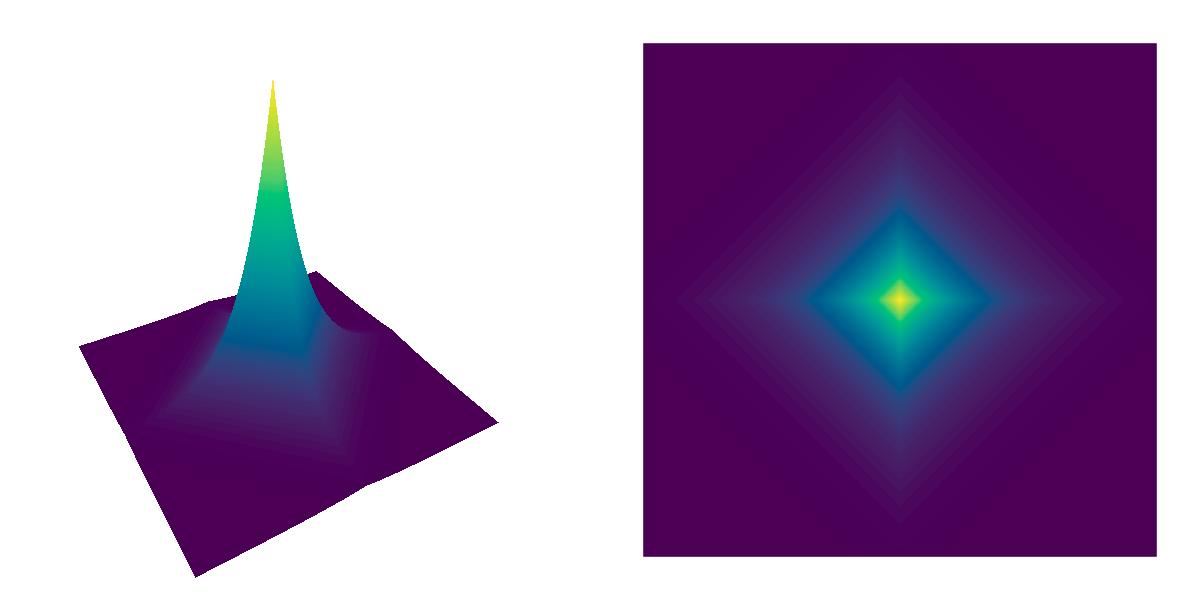
\includegraphics[width=.9\textwidth]{./figures/de.jpg}
    \caption{Two dimensional double exponential density with $\lambda=1$.}
    \label{fig:double_exp}
\end{figure}

It follows that the prior distribution for $\beta$ is given by,
\begin{equation} \label{eq:prior} 
    \Pi(\beta | z) = \bigotimes_{k=1}^{M} \left[ 
    z_k \Psi(\beta_{G_k}; \lambda) + (1-z_k)\delta_0(\beta_{G_k})
\right]
\end{equation}
where $z = (z_1, \dots, z_M)$ and $\otimes$ is the product measure.


\red{
Regarding $\tau^2$, there are many popular choices that a practitioner may wish to use, for example:
\begin{itemize}
    \itemsep0em
    \item \textit{Locally uniform}, wherein $\tau^2 \sim U(0, 1/\varepsilon)$ for a small positive $\varepsilon$.
    \item \textit{Inverse-Gamma}, wherein $\tau^2 \sim \Gamma^{-1}(a, b)$, where $\Gamma^{-1}$ denotes an inverse-Gamma distribution with shape $a$ and scale $b$, with a common choice for each being $a=b=\varepsilon$, where $\varepsilon$ is a small positive constant around $0.001$.
\end{itemize}
In the meantime, we place do not place a prior on $\tau^2$ and assume it is known.
}

\subsection{Posterior}

The posterior density is given by,
\begin{equation} \label{eq:posterior} 
d\Pi(\beta | \D) = \Pi_D^{-1} e^{\ell(\D; \beta)} d\Pi(\beta)
\end{equation}
where $\Pi_\D = \int_{\R^{p}} e^{\ell(\D; \beta)} d\Pi(\beta)$ is a normalization constant and $\ell(\D; \beta)$ is the log-likelihood function. (This isn't exactly correct, we still need to integrate our the $z$ terms and re-write the prior).


\subsection{Variational Family}

In turn, our aim is to approximate \eqref{eq:posterior} by a member of a tractable family of distributions, referred to as the variational family. We have chosen the family,
\begin{equation}
    \Q = \left\{ Q = \Gamma^{-1}(a, b) \bigotimes_{k=1}^M \left[ 
    \gamma_k\ N\left(\mu_{G_k}, \diag( \sigma_{G_k}) \right) + (1-\gamma_k) \delta_0
\right] \right\}
\end{equation}
where $N(\mu, \Sigma)$ denotes the multivariate Normal distribution with mean parameter $\mu$ and covariance $\Sigma$. In turn the variational posterior is given by solving,
\begin{equation} \label{eq:optim} 
\tilde{\Pi} = \underset{Q \in \Q}{\argmin}\ \KL\left( Q \| \Pi(\cdot |\D) \right)
\end{equation}
and is used in subsequent analysis as a proxy for the true posterior.


% ----------------------------------------
% ----------------------------------------
% ----------------------------------------
\section{Co-ordinate ascent algorithm}

Throughout our derivation we exploit the group independence structure within the prior and variational distribution, allowing the Radon-Nikodym derivative of $Q$ with respect to the prior $\Pi$ to be expressed as,
\begin{equation}
    \frac{dQ}{d\Pi}(\beta) = \prod_{k=1}^{M} \frac{dQ_k}{d\Pi_k} (\beta_{G_k})
\end{equation}

Consider, the optimization problem \eqref{eq:optim} and recall the definition of the KL divergence \eqref{eq:kl}, it follows that
\begin{align}
    \KL(Q \| \Pi(\cdot | \D)) 
    = &\ \E_{Q} \left[ \log \frac{dQ}{d\Pi(\dot | \D)} \right] 
    = \E_Q \left[ \log \frac{\Pi_\D dQ}{e^{\ell(\D; \beta)} d\Pi} \right] \nonumber \\
    =&\ \E_Q \left[ -\ell(\D; \beta) + \log \frac{dQ}{d\Pi} \right] + \log \Pi_\D \label{eq:opt} 
\end{align}
As optimization of the objective \eqref{eq:optim} is invariant to constant terms, to simplify upcoming expressions we write them as $C$ (the value of which may change line by line).

\subsection{Updates of $\mu_{G_k}$ and $\sigma_{G_k}$}

In order to update $\mu_{G_k}$ and $\sigma_{G_k}$ we must assume that the group takes a non-zero value, i.e. $z_k =1$. Hence, %
{\allowdisplaybreaks
\begin{align}
\E_{Q  | z_K = 1} & \left[ 
    - \ell(\D; \beta) + \log \frac{dQ}{d\Pi}(\beta) 
\right]  \nonumber \\
= &\
    \E_{Q | z_K = 1} \left[ 
	- \ell(\D; \beta) + \log \prod_{k=1}^M \frac{dQ_k}{d\Pi_k}(\beta_{G_k})
    \right] \nonumber \\
= &\
    \E_{Q | z_K = 1} \left[ 
	- \ell(\D; \beta) 
	+ \log \frac{dQ_K}{d\Pi_K}(\beta_{G_K})
	+ \log \prod_{k \neq K} \frac{dQ_k}{d\Pi_k}(\beta_{G_k})
    \right] \nonumber \\
= &\
    \E_{Q | z_K = 1} \left[ 
	\frac{1}{2\tau^2} \| y - X \beta \|^2
	+ \log \frac{dQ_K}{d\Pi_K}(\beta_{G_K})
    \right] + C \nonumber \\
= &\
    \E_{Q | z_K = 1} \left[ 
	\frac{1}{2\tau^2} \bigg\{ 
	    \| X \beta \|^2 - 2 \langle y, X\beta \rangle 
	\bigg\}
	+ \log \frac{dQ_K}{d\Pi_K}(\beta_{G_K})
    \right] + C \nonumber \\
= &\
    \E_{Q | z_K = 1} \left[ 
	\frac{1}{2\tau^2} \left\{ 
	    \tr \left( X^\top X \beta \beta^\top \right) 
	    - 2 \sum_{k=1}^M \langle y, X_{G_k} \beta_{G_k} \rangle 
	\right\}
	+ \log \frac{dQ_K}{d\Pi_K}(\beta_{G_K})
    \right] + C \nonumber \\
= &\
    \E_{Q | z_K = 1} \left[ 
	\frac{1}{2\tau^2} \tr \left( X^\top X \beta \beta^\top \right) 
	- \frac{1}{\tau^2} \langle y, X_{G_K} \beta_{G_K} \rangle 
	+ \log \frac{dQ_K}{d\Pi_K}(\beta_{G_K})
    \right] + C \label{eq:mu_sigma_1}
\end{align}
} %
where $\tr(\cdot)$ denotes the trace of a matrix and $C$ is a constant term whose value does not depend on $\mu_{G_K}$ or $\sigma_{G_K}$ (and may change line by line).

Consider the matrix $ X^\top X \beta \beta^\top \in \R^{p \times p} $, using the fact that $\left( X^\top X \beta \beta^\top \right)_{ii} = \sum_{j=1}^{p} (X^\top X)_{ji} \beta_j \beta_i $ for $i,j = 1, \dots, p$, we have
\begin{align}
    \E_{Q | z_K = 1} & \left[ 
	\tr \left( X^\top X \beta \beta^\top \right) 
    \right]
=
    \E_{Q | z_K = 1} \left[ 
	\sum_{i=1}^p \sum_{j=1}^{p} (X^\top X)_{ji} \beta_j \beta_i 
    \right] \nonumber \\
=&\
    \sum_{i=1}^p \sum_{j=1}^{p} (X^\top X)_{ji} 
    \E_{Q | z_K = 1} \left[ \beta_j \beta_i \right] 
    \nonumber \\
=&\
    \sum_{i \in G_K} \left(
	\sum_{j=1}^{p} (X^\top X)_{ji} 
	\E_{Q | z_K = 1} \left[ \beta_j \beta_i \right]
    \right)
+
    \sum_{i \in G_K^c} \left(
	\sum_{j=1}^{p} (X^\top X)_{ji} 
	\E_{Q | z_K = 1} \left[ \beta_j \beta_i \right] 
    \right)
    \nonumber \\
=&\
    \sum_{i \in G_K} \left( 
	\sum_{j \in G_K} (X^\top X)_{ji} 
	    \E_{Q | z_K = 1} \left[ \beta_j \beta_i \right] 
	+ 
	\sum_{j \in G_K^c} (X^\top X)_{ji} 
	    \E_{Q | z_K = 1} \left[ \beta_j \beta_i \right] 
    \right ) \nonumber \\
+&\ 
    \sum_{i \in G_K^c} \left( 
	\sum_{j \in G_K} (X^\top X)_{ji} 
	    \E_{Q | z_K = 1} \left[ \beta_j \beta_i \right] 
	+ 
	\sum_{j \in G_K^c} (X^\top X)_{ji} 
	    \E_{Q | z_K = 1} \left[ \beta_j \beta_i \right] 
    \right ) \nonumber \\
=&\
    \sum_{i \in G_K} \left( 
	\sum_{j \in G_K} (X^\top X)_{ji} 
	    \E_{Q | z_K = 1} \left[ \beta_j \beta_i \right] 
	+ 
	2 \sum_{j \in G_K^c} (X^\top X)_{ji} 
	    \E_{Q | z_K = 1} \left[ \beta_j \beta_i \right] 
    \right ) + C \nonumber
\end{align}
Consider, $ \E_{Q | z_K = 1} \left[ \beta_j \beta_i \right] $ and note $\cov(\beta_j, \beta_i) = \E\left[ \beta_j \beta_i \right] - \E \left[\beta_j \right] \E \left[ \beta_i \right]$, the previous display results in three cases
\begin{equation}
    \E_{Q | z_K = 1} \left[ \beta_j \beta_i \right] = \begin{cases}
	\sigma_{j}^2 + \mu_{j}^2 	& \quad i,j \in G_K, i=j \\
	\mu_{j}\mu_{i} 			& \quad i,j \in G_K, i \neq j \\
	\gamma_J \mu_{j}\mu_{i} 	& \quad i \in G_K, j \in G_J, J \neq K
    \end{cases}
\end{equation}

The second term in \eqref{eq:mu_sigma_1} is straightforward and is given as,
\begin{equation} \label{eq:mu_sigma_term_2}
    \E_{Q | z_K = 1} \left[ \langle y, X_{G_K} \beta_{G_K} \rangle  \right]
=   
    \langle y, X_{G_K} \E_{Q | z_K = 1} \left[ \beta_{G_K} \right] \rangle   
=
    \langle y, X_{G_K} \mu_{G_K} \rangle  
\end{equation}

Finally, the third term in \eqref{eq:mu_sigma_1} is given as,
\begin{align}
    \E_{Q | z_K = 1 } & \left[ \log \frac{dQ_K}{d\Pi_K} (\beta_{G_K}) \right]
    \nonumber \\
= &\
    \E_{Q | z_K = 1 } \left[ 
	\log \frac
	{\prod_{j \in G_K} \left( 2 \pi \sigma_j^2 \right)^{-1/2} \exp \left\{ -(2\sigma^2_{j})^{-1}(\beta_{j} - \mu_j )^2 \right\}}
	{C_K \lambda^{m_K} \exp\left( - \lambda \| \beta_{G_K} \| \right)}
    \right] \nonumber \\
= &\
    \E_{Q | z_K = 1 } \left[ 
	\lambda \| \beta_{G_K} \|
	- \sum_{j \in G_K} \left( 
	    \log{\sigma_j} 
	    + \frac{1}{2\sigma_j^2} (\beta_{j} - \mu_j)^2
	\right)
    \right] + C \nonumber \\
= &\
    \lambda \E_{Q | z_K = 1 } \left[ 
	\| \beta_{G_K} \|
    \right] 
    - \sum_{j \in G_K} \log{\sigma_j} 
    - \frac{m_K}{2} 
    + C 
    \label{eq:mu_simga_term_3}
\end{align}
Evaluating the remaining expectation in \eqref{eq:mu_simga_term_3} is non-trivial, in turn we derive an upper bound using Jensen's inequality,
\begin{equation} \label{eq:mu_sigma_upper}
    \E_{Q | z_K = 1 } \left[ 
	\| \beta_{G_K} \|
    \right] 
    % \E_{Q | z_K = 1 } \left[ 
	% \left( \sum_{j \in G_K} \beta_{j}^2 \right)^{1/2}
    % \right] 
    % \nonumber \\
\leq
    \left( \sum_{j \in G_K} 
	\E_{Q | z_K = 1 } \left[ \beta_{j}^2 \right] 
    \right)^{1/2} 
=
    \left( \sum_{j \in G_K} 
	\sigma_j^2 + \mu_j^2
    \right)^{1/2} 
\end{equation}
Putting these components together gives
\begin{equation} \label{eq:mu_sigma_main}
\begin{aligned}
    \E_{Q  | z_K = 1} & \left[ 
	- \ell(\D; \beta) + \log \frac{dQ}{d\Pi}(\beta) 
    \right]  \\
\leq &\
    \frac{1}{2\tau^2} 
    \sum_{i \in G_K} \left( 
	    (X^\top X)_{ii} (\sigma_i^2 + \mu_i^2)
	+
	\sum_{j \in G_K, j\neq i} 
	    (X^\top X)_{ji} \mu_j \mu_i
    \right ) \\
+ &\
    \frac{1}{\tau^2} 
    \sum_{i \in G_K} \left( 
    \sum_{j \in G_K^c} (X^\top X)_{ji} 
	\gamma_{J} \mu_j \mu_i
    \right )
-
    \frac{1}{\tau^2}
    \langle y, X_{G_K} \mu_{G_K} \rangle   \\
- &\
    \sum_{i \in G_K} \log{\sigma_i}
+
    \lambda \left( \sum_{i \in G_K} 
	\sigma_i^2 + \mu_i^2
    \right)^{1/2} + C
\end{aligned}
\end{equation}

\subsubsection{Group-wise update for $\mu_{G_K}$}

Re-writing the RHS of \eqref{eq:mu_sigma_main} in terms of $\mu_{G_K}$, we have
\begin{equation} \label{eq:mu_gk}
\begin{aligned}
    \frac{1}{2\tau^2} 
    \mu_{G_K}^\top X_{G_K}^\top X_{G_K} \mu_{G_K}
+
    \frac{1}{\tau^2} 
    \sum_{J \neq K} 
	\gamma_J \mu_{G_K}^\top X_{G_K}^\top X_{G_J} \mu_{G_J} 
-
    \frac{1}{\tau^2}
    \langle y, X_{G_K} \mu_{G_K} \rangle \\
+
    \lambda \left( \sigma_{G_K}^\top \sigma_{G_K} + \mu_{G_K}^\top \mu_{G_K} \right)^{1/2} + C
\end{aligned}
\end{equation}

\textbf{Insight into the update of $\mu_{G_K}$}

Using the fact that $ \left( \sum_{j \in G_K} \sigma_j^2 + \mu_j^2 \right)^{1/2} \leq 1 + \sum_{j \in G_K} \sigma_j^2 + \mu_j^2 $ we can upper bound \eqref{eq:mu_gk}.
\begin{equation} \label{eq:mu_gk_upper}
\begin{aligned}
    \frac{1}{2\tau^2} 
    \| X_{G_K} \mu_{G_K} \|^2
+
    \frac{1}{\tau^2} 
    \sum_{J \neq K} 
	\gamma_J \mu_{G_K}^\top X_{G_K}^\top X_{G_J} \mu_{G_J} 
-
    \frac{1}{\tau^2}
    \langle y, X_{G_K} \mu_{G_K} \rangle
+
    \lambda \| \mu_{G_K} \|^2 + C
\end{aligned}
\end{equation}
And in turn \eqref{eq:mu_gk_upper} is minimized by
\begin{equation} \label{eq:mu_gk_min}
    \hat{\mu}_{G_K} = \Xi^{-1} X_{G_K}^\top y - \Xi^{-1} \sum_{J \neq K} \gamma_J X_{G_K}^\top X_{G_J} \mu_{G_J}    
\end{equation}
where $\Xi = X_{G_K}^\top X_{G_K} + 2 \lambda \tau^2 I_{m_K}$. 

Let $P := (X_{G_K}^\top X_{G_K} + 2 \lambda \tau^2 I_{m_K})^{-1} X_{G_K}^\top $ and the prediction of $y$ from $\mu_{G_J}$ as $\hat{y}_{G_J} = X_{G_J} \mu_{G_J}$, then we can re-express \eqref{eq:mu_gk_min} as
\begin{equation}
\hat{\mu}_{G_K} = P(y - \sum_{J \neq K} \gamma_J \hat{y}_{G_J})
\end{equation}
In other words the minimizer $\hat{\mu}_{G_K}$ seeks a vector that explains the remaining signal in $y$ given the signal explained by $\sum_{J \neq K} \gamma_J \hat{y}_{G_J}$, for example, consider the extreme case, $y - \sum_{J \neq K} \gamma_J \hat{y}_{G_J} = 0_n$ (the n-dimensional zero vector), then the resulting minimizer $\hat{\mu}_{G_K} = 0_{m_K}$. 

It turns out, updating using \eqref{eq:mu_gk_min} doesn't work that well in practise, in fact, using optimization routines to minimize \eqref{eq:mu_gk} leads to better results in less time.


\subsubsection{Group-wise update for $\sigma_{G_K}$}

Re-writing the RHS of \eqref{eq:mu_sigma_main} in terms of $\sigma_{G_K}$, we have
\begin{equation} \label{eq:sig_gk}
\begin{aligned}
    \sum_{i \in G_K} \left( 
    \frac{1}{2\tau^2} 
	    (X^\top X)_{ii} \sigma_i^2
-
    \log{\sigma_i}
    \right )
+
    \lambda \left( \sum_{i \in G_K} 
	\sigma_i^2 + \mu_i^2
    \right)^{1/2} + C
\end{aligned}
\end{equation}

\subsection{Updates for $\gamma_K$}

Similarly for $\gamma_K$ we evaluate the expectation with respect to $Q$, however without conditioning on the group being non-zero.
{\allowdisplaybreaks
\begin{align}
    \E_{Q} & \left[ 
	- \ell(\D; \beta) + \log \frac{dQ}{d\Pi}(\beta) 
    \right]  \nonumber \\
= &\
    \E_{Q} \left[ 
	- \ell(\D; \beta) 
	+ \I_{\{z_K = 1\}} \log \frac{\gamma_K dN_K}{\bar{w} d\Psi_K}(\beta_{G_K}) 
	+ \I_{\{z_K = 0\}} \log \frac{1 - \gamma_K}{1 - \bar{w}}
    \right] + C \nonumber \\
=&\
    \frac{1}{2\tau^2} 
    \sum_{i \in G_K} \left( 
	\sum_{j \in G_K} (X^\top X)_{ji} 
	    \E_{Q} \left[ \beta_j \beta_i \right] 
	+ 
	2 \sum_{j \in G_K^c} (X^\top X)_{ji} 
	    \E_{Q} \left[ \beta_j \beta_i \right] 
    \right ) \nonumber \\
- &\
    \frac{1}{\tau^2} \langle y, X_{G_K} \E_Q\left[\beta_{G_K} \right] \rangle 
-
    \frac{\gamma_K}{2} \sum_{j \in G_K} \log \left( 2 \pi \sigma_j^2 \right)
-
    \gamma_K \log(C_K )
    \nonumber \\
- &\
    \gamma_K m_K \log (\lambda) 
+ 
    \E_{Q} \left[ 
	\I_{\{z_K=1\}} \left(
	\lambda \| \beta_{G_K} \|
	- \sum_{j \in G_K}
	    \frac{1}{2\sigma_j^2} (\beta_{j} - \mu_j)^2
	\right)
    \right]  \nonumber \\ 
+ &\
    \gamma_K \log \frac{\gamma_K}{\bar{w}}
    + (1 - \gamma_K) \log \frac{1 - \gamma_K}{1 - \bar{w}}
+ C \nonumber
\end{align}
}
Noting $\E_Q \left[ \beta_{G_K} \right] = \gamma_K \mu_{G_K} $ and
\begin{equation}
    \E_{Q} \left[ \beta_j \beta_i \right] = \begin{cases}
	\gamma_K (\sigma_{j}^2 + \mu_{j}^2) 	& \quad i,j \in G_K, i=j \\
	\gamma_K \mu_{j}\mu_{i} 		& \quad i,j \in G_K, i \neq j \\
	\gamma_K \gamma_J \mu_{j}\mu_{i} 	& \quad i \in G_K, j \in G_J, J \neq K
    \end{cases}
\end{equation}
and
\begin{equation}
    \E_Q \left[ \I_{\{z_K = 1\}} \| \beta_{G_K} \| \right] = 
    \gamma_K \E_{N_K} \left[ \| \beta_{G_K} \| \right]
    \leq \gamma_K \left( \sum_{j \in G_K} \sigma^2_j + \mu^2_j \right)^{1/2}
\end{equation}
Substituting these expressions into the previous display gives,
\begin{equation*}
\begin{aligned}
    \E_{Q} & \left[ 
	- \ell(\D; \beta) + \log \frac{dQ}{d\Pi}(\beta) 
    \right]  \\
\leq &\
    \frac{\gamma_K}{2\tau^2}
    \sum_{i \in G_K} \left( 
	    (X^\top X)_{ii} (\sigma_i^2 + \mu_i^2)
	+
	\sum_{j \in G_K, j\neq i} 
	    (X^\top X)_{ji} \mu_j \mu_i
    \right ) \\
+ &\
    \frac{\gamma_K}{\tau^2}
    \sum_{i \in G_K} \left( 
    \sum_{j \in G_K^c} (X^\top X)_{ji} 
	\gamma_{J} \mu_j \mu_i
    \right )
-
    \frac{\gamma_K}{\tau^2} \langle y, X_{G_K} \mu_{G_K} \rangle \\
- &\
    \frac{\gamma_K}{2} \sum_{j \in G_K} \log \left( 2 \pi \sigma_j^2 \right) 
-
    \gamma_K \log(C_K )
-
    \gamma_K m_K \log (\lambda) 
+
    \lambda \gamma_K \left( \sum_{j \in G_K} 
	\sigma_j^2 + \mu_j^2
    \right)^{1/2} \\
- &\
    \frac{\gamma_K m_K}{2} 
% + 
    % \gamma_K \sum_{j \in G_K} \frac{\mu_j^2}{2 \sigma_j^2}
+ 
    \gamma_K \log \frac{\gamma_K}{\bar{w}}
+ 
    (1 - \gamma_K) \log \frac{1 - \gamma_K}{1 - \bar{w}}
+ C
\end{aligned}
\end{equation*}
Differentiating the RHS of the previous display with respect to $\gamma_K$, setting to zero and re-arranging givens the update equation for $\gamma_K$, formally,
\begin{equation} \label{eq:update_gamma} 
\begin{aligned}
    \log &\ \frac{\gamma_K}{1-\gamma_K} = 
    \log \frac{\bar{w}}{1-\bar{w}}
+ 
    \frac{m_K}{2}  
+
    \frac{1}{\tau^2} \langle y, X_{G_K} \mu_{G_K} \rangle  \\
+ &\ 
    \frac{1}{2} \sum_{j \in G_K} \log \left( 2 \pi \sigma_j^2 \right)
+
    \log(C_K )
+
    m_K \log (\lambda)
-
\Bigg\{ 
    \lambda \left( \sum_{j \in G_K} 
	\sigma_j^2 + \mu_j^2
    \right)^{1/2}  \\
+ &\
    \frac{1}{2\sigma^2}
    \sum_{i \in G_K} \left( 
    (X^\top X)_{ii} \sigma_i^2
    +
    \sum_{j \in G_K} 
	(X^\top X)_{ji} \mu_j \mu_i
    % \right )
+
    % \frac{1}{\sigma^2}
    % \sum_{i \in G_K} \left( 
    2 \sum_{j \in G_K^c} (X^\top X)_{ji} 
	\gamma_{J} \mu_j \mu_i
    \right )
\Bigg\}
\end{aligned}
\end{equation}


\subsection{Evidence Lower Bound}

The evidence lower bound, acts as a lower bound for the model evidence $\Pi_\D$, and follows from the definition of the KL divergence,
\begin{align*}
 & 0 \leq \KL(Q \| \Pi(\cdot | \D)) = \E_Q \left[ \Pi_\D - \ell(\D; \beta) - \log \frac{d\Pi}{dQ} (\beta) \right] \\
    \implies & \E_Q \left[ \ell(\D; \beta) + \log \frac{d\Pi}{dQ} (\beta) \right] \leq \Pi_\D
\end{align*}
Formally, the ELBO is defined as,
\begin{equation}
   \L(\D) = \E_Q \left[ \ell(\D; \beta) + \log \frac{d\Pi}{dQ}(\beta) \right]
\end{equation}
In effect, maximizing the ELBO is equivalent to minimizing $\KL(Q \| \Pi(\cdot | \D)) $, i.e. solving \eqref{eq:optim}. Often the ELBO is used to assess the convergence of co-ordinate ascent algorithms, but can also act as a goodness of fit measure.

For our model the ELBO is given as
\begin{equation} \label{eq:elbo} 
\begin{aligned}
    \L(\D) &= 
- 
    \frac{n}{2} \log(2 \pi \tau^2) 
- 
    \frac{1}{2\tau^2} \left( \| y \|^2  + \sum_{i=1}^p \sum_{j=1}^p (X^\top X)_{ji} \E_Q \left[ \beta_j \beta_i \right] \right)\\
+& 
    \sum_{K=1}^M \bigg(  
\frac{1}{\tau^2} \gamma_K \langle y, X_{G_K} \mu_{G_K} \rangle
+
    \frac{\gamma_K}{2} \sum_{j \in G_K} \left( \log( 2 \pi \sigma_j^2) \right)
+
    \gamma_K \log(C_K)
+ 
    \frac{\gamma_K m_K}{2} \\
+ &
    \gamma_K m_K \log (\lambda)
-
    \E_Q \left[ \I_{z_K =1} \lambda \| \beta_{G_K} \| \right]
-
    \gamma_K \log \frac{\gamma_K}{\bar{w}}
-
    (1-\gamma_K) \log \frac{1 - \gamma_K}{1 - \bar{w}}
\bigg)
\end{aligned}
\end{equation}
where the expectation $\E_Q \left[ \beta_i \beta_j \right]$ is defined earlier. Given $\E_Q \left[ \I_{\{z_K = 1\}} \lambda \| \beta_{G_K} \| \right] $ does not have a closed form expression, Monte-Carlo integration to evaluate it.

\subsection{Updating $\tau$}

As of yet we have not placed a prior on $\tau^2$ or considered updating $\tau^2$ as part of our co-ordinate ascent algorithm. This is because, under an independent prior for $\tau^2$ and independent factorization in our mean-field variational family, we can update our existing equations for $\mu_{G_K}, \sigma_{G_K}$, $\gamma_K$ and ELBO to include this modelling assumption.

To demonstrate, we opt to use an inverse Gamma prior, predominately because it is a popular choice amongst practitioners \citep{Browne2006}. Formally, we have,
\begin{equation}
    \tau^2 \sim \Gamma^{-1}(a, b)
\end{equation}

Extending our prior \eqref{eq:prior} to include this modelling assumption for $\tau^2$, we have,
\begin{equation}
    \Pi'(\beta, \tau^2) = \Pi(\tau^2) \Pi(\beta) = \Gamma^{-1}(\tau^2; a, b) \Pi(\beta)
\end{equation}
Similarly, extending our variational family with respect to $\tau^2$, we have,
\begin{equation}
    \Q' = \{ \Gamma^{-1}(\tau^2; a', b') : a' > 0, b' > 0 \} \times \Q
\end{equation}
where we denote,
\begin{equation}
    Q' = \Gamma^{-1}(\tau^2; a', b') \otimes Q(\beta) \in \Q' 
\end{equation}

Given these extension, our original optimization problem \eqref{eq:opt} is extended to be
\begin{equation}
    \E_{Q'} \left[ -\ell(\D; \beta) + \log \frac{dQ'}{d\Pi'} \right] = 
    \E_{Q'} \left[ -\ell(\D; \beta) + \log \frac{dQ}{d\Pi} + \log \frac{d\Gamma^{-1}(a', b')}{d \Gamma^{-1}(a, b)}(\tau^2)\right]
\end{equation}
Consequently, when deriving the new update equations for $\mu_{G_K}, \sigma_{G_K}$ and $\gamma_K$, this new term $ \E [ \log \frac{d\Gamma^{-1}}{d\Gamma^{-1}} ] $ is a constant. Therefore, we need only replace all occurrences of $1/\tau^2$ in our old update equations with $\E_{\Gamma^{-1}} [ 1 / \tau^2 ] $. Regarding the ELBO we do the same, however we also include the term $ \E_{\Gamma^{-1}} [ \log \frac{d\Gamma^{-1}}{d\Gamma^{-1}}] $.

Finally, to update the parameters $a'$ and $b'$ we re-write \eqref{eq:opt} as a function of $a'$ and $b'$,
\begin{align*}
    \E_{Q'} & \left[ -\ell(\D; \beta) + \log \frac{dQ'}{d\Pi'} \right]
=  
    \E_{Q'} \left[
-
    \ell(\D; \beta)
+   
    \log \frac{d\Gamma^{-1}(a', b')}{d \Gamma^{-1}(a, b)}(\tau^2)\right] 
+
    C \\  
= &\
\E_{Q'} \left[ 
    \frac{n}{2}\log(\tau^2) 
+ 
    \frac{1}{2\tau^2} \| y - X \beta \|^2 
+
    (a - a') \log(\tau^2)
+
    \frac{b' - b}{\tau^2}
\right] + C \\
= &\
\E_{Q'} \left[ 
    \left( \frac{n}{2} + a - a' \right) \log(\tau^2) 
+ 
    \frac{1}{2\tau^2} \left( \| y \|^2
    - 2 \langle y, X \beta \rangle
    + \| X \beta \|^2
    \right)
+
    \frac{b' - b}{\tau^2}
\right] + C \\  
= &\
\E_{\Gamma^{-1}} \left[ 
    \left( \frac{n}{2} + a - a' \right) \log(\tau^2) 
+
    \frac{b' - b}{\tau^2}
\right] \\
+ &\ 
    \E_{\Gamma^{-1}} \left[ \frac{1}{2\tau^2} \right]
    \left( \| y \|^2 
    - 2 \langle y, X \E_Q \left[ \beta \right] \rangle
+  \sum_{i=1}^p \sum_{j=1}^p (X^\top X)_{ji} \E_Q \left[ \beta_j \beta_i \right]
    \right)
+ C \\  
= &\
    \left( \frac{n}{2} + a - a' \right) \left( \log(b') + \kappa(a') \right)
+
    a' - \frac{a'b}{b'}
    \\
+ &\ 
    \frac{a'}{2b'}
    \left( \| y \|^2 
- 
    2 \sum_{K=1}^M \gamma_{G_K} \langle y, X_{G_K} \mu_{G_K} \rangle
+  
    \sum_{i=1}^p \sum_{j=1}^p (X^\top X)_{ji} \E_Q \left[\beta_j \beta_i \right]
    \right) 
+ C
\end{align*}
Where we have used the fact $\E_{\Gamma^2{-1}} [ \log(\tau^2) ] =  \log(b') + \kappa(a') $ and $\E_{\Gamma^{-1}} [ 1 / \tau^2 ] = a' / b' $, where $\kappa(a')$ is the digamma function. Writing the previous display as a function of $a'$ we have
\begin{equation} \label{eq:a_update}
\begin{aligned}
    & \left( \frac{n}{2} + a - a' \right) \kappa(a')
+
    a' - \frac{a'b}{b'}
+  \\
&
    \frac{a'}{2b'}
    \left( \| y \|^2 
- 
    2 \sum_{K=1}^M \gamma_{G_K} \langle y, X_{G_K} \mu_{G_K} \rangle
+  
    \sum_{i=1}^p \sum_{j=1}^p (X^\top X)_{ji} \E_Q \left[\beta_j \beta_i \right]
    \right) 
+ C
\end{aligned}
\end{equation}
Similarly, for $b'$ we have,
\begin{equation} \label{eq:b_opt}
\begin{aligned}
    & \left( \frac{n}{2} + a - a' \right) \log(b')
- 
    \frac{a'b}{b'}
+  \\
&
    \frac{a'}{2b'}
    \left( \| y \|^2 
- 
    2 \sum_{K=1}^M \gamma_{G_K} \langle y, X_{G_K} \mu_{G_K} \rangle
+  
    \sum_{i=1}^p \sum_{j=1}^p (X^\top X)_{ji} \E_Q \left[\beta_j \beta_i \right]
    \right) 
+ C
\end{aligned}
\end{equation}
As there is no closed form minimizer of \eqref{eq:a_update} optimization routines can be used, whereas the minimizer of \eqref{eq:b_opt} is given by,
\begin{equation*}
    b'_{\min} = 
\frac{a'}{2}
\frac{n/2 +a - a'}
{
    \| y \|^2 
- 
    2 \sum_{K=1}^M \gamma_{G_K} \langle y, X_{G_K} \mu_{G_K} \rangle
-
    2b
+  
    \sum_{i=1}^p \sum_{j=1}^p (X^\top X)_{ji} \E_Q \left[\beta_j \beta_i \right]
}
\end{equation*}



\newpage
\section{Simulation study}

...



\newpage
\bibliography{refs.bib}

\appendix
\numberwithin{equation}{section}


\section{Definitions}
\textbf{Definition} \textit{Kullback-Leibler divergence}.\\ Let $Q$ and $P$ be probability measures on $\Xc$, such that $ Q $ is absolutely continuous with respect to $P$, then the Kullback-Leibler divergence is defined as,
\begin{equation}\label{eq:kl}
\KL(Q \| P) = \int_{\Xc} \log \left( \frac{dQ}{dP} \right) dQ
\end{equation}
where $dQ/dP$ is the Radon-Nikodym derivative of $Q$ with respect to $P$.


\section{Co-ordinate ascent algorithm}

\subsection{Element-wise update equations}

\textbf{Updates for $\mu_{G_K}$}
\begin{equation} \label{eq:mu_update}
\begin{aligned}
    f(\mu_i; & \mu_{-i}, \sigma, \gamma) :=\
    \frac{1}{2\tau^2} \left(
	(X^\top X)_{ii} \mu_i^2 + 
	\sum_{j \in G_K, j\neq i} (X^\top X)_{ji} \mu_j \mu_i
    \right) \\
+ &\
    \frac{1}{\tau^2} \left(
	\bigg( \sum_{j \in G_K^c} (X^\top X)_{ji} \gamma_{J} \mu_j \mu_i \bigg) -
	\mu_i \langle y, X_{:i} \rangle   
    \right)
+
    \lambda \left( \sum_{j \in G_K} 
	\sigma_j^2 + \mu_j^2
    \right)^{1/2} + C
\end{aligned}
\end{equation}
The above expression in turn is minimized via optimization routines.

Using the fact that $ \left( \sum_{j \in G_K} \sigma_j^2 + \mu_j^2 \right)^{1/2} \leq 1 + \sum_{j \in G_K} \sigma_j^2 + \mu_j^2 $, we can obtain a looser upper bound on \eqref{eq:mu_sigma_main} and the resulting expression we need to minimize,
\begin{equation}
\begin{aligned}
    f_2(\mu_i; & \mu_{-i}, \sigma, \gamma) :=\
    \frac{1}{2\tau^2} \left(
	(X^\top X)_{ii} \mu_i^2 + 
	\sum_{j \in G_K, j\neq i} (X^\top X)_{ji} \mu_j \mu_i
    \right) \\
+ &\
    \frac{1}{\tau^2} \left(
	\sum_{j \in G_K^c} \left[ (X^\top X)_{ji} \gamma_{J} \mu_j \mu_i \right] -
	\mu_i \langle y, X_{:i} \rangle   
    \right)
+
    \lambda \mu_i^2 + C
\end{aligned}
\end{equation}
which in turn in minimized when
\begin{equation} \label{eq:mu_analytic}
    \mu_i =
    - \frac{
	\left(\sum_{j \in G_K^c} (X^\top X)_{ji} \gamma_{J} \mu_j \right) +
	\frac{1}{2} \left(\sum_{j \in G_K, j\neq i} (X^\top X)_{ji} \mu_j \right)-
	\langle y, X_{:i} \rangle 
    }{
	(X^\top X)_{ii} +
	2 \tau^2 \lambda 
    }
\end{equation}

Interestingly, if we assume the columns of $X$ are orthogonal, i.e. $ (X^\top X)_{ij} = 0$ for $i \neq j$, and $\lambda = 0$, then \eqref{eq:mu_analytic} can be written as
\begin{equation}
    \mu_i^{\text{ols}} = (X^\top X)_{ii}^{-1} (X_{:i})^\top y
\end{equation}
which we recognize as the ordinary least squares estimator under an orthogonal design. Similarly, when $\lambda > 0$, the minimizer is given by
\begin{equation}
    \mu_i^{\text{rr}} := \left((X^\top X)_{ii} + 2\tau^2 \lambda \right)^{-1} (X_{:i})^\top y
\end{equation}
which we recognize as the solution under the ridge penalty. It follows that the minimizer \eqref{eq:mu_analytic} is given by a ridge term under the assumption of an orthogonal design and some additional term, formally,
\begin{equation}
    \mu_i = \mu_i^{\text{rr}} - \frac{
	\left(\sum_{j \in G_K^c} (X^\top X)_{ji} \gamma_{J} \mu_j \right) +
	\frac{1}{2} \left(\sum_{j \in G_K, j\neq i} (X^\top X)_{ji} \mu_j \right)
    }{
	(X^\top X)_{ii} +
	2 \tau^2 \lambda 
    }
\end{equation}

\textbf{Updates for $\sigma_{G_K}$}
\begin{equation}
\begin{aligned}
    g(\sigma_i;& \mu, \sigma_{-i}, \gamma) :=\
    \frac{1}{2\tau^2} (X^\top X)_{ii} \sigma_i^2
-
    \log{\sigma_i}
+
    \lambda \left( \sum_{j \in G_K} 
	\sigma_j^2 + \mu_j^2
    \right)^{1/2} + C
\end{aligned}
\end{equation}
As before, under the looser upper bound we have,
\begin{equation}
    g_2 (\sigma_i; \mu, \sigma_{-i}, \gamma) :=\
    \frac{1}{2\tau^2} (X^\top X)_{ii} \sigma_i^2
-
    \log{\sigma_i}
+
    \lambda \sigma_i^2 + C
\end{equation}
which is minimized when,
\begin{equation}
    \sigma_i = \left( \frac{(X^\top X)_{ii}}{\sigma^2} + 2 \lambda \right)^{-1/2}
\end{equation}
which we notice does not depend on the other parameters and in turn can be used to initialize $\sigma_i$.



\end{document}
